\documentclass[11pt,dvipsnames]{article}
%\usepackage[dvipdfm]{graphicx}
\usepackage{graphicx}
\usepackage{debulletin,times}
\usepackage{color}
\usepackage{xcolor}
\usepackage{xspace}
\usepackage{wrapfig}
\usepackage{enumitem}
\usepackage{tabularx}

\usepackage{caption}
\usepackage{float}

\newcommand\setrow[1]{\gdef\rowmac{#1}#1\ignorespaces}
\setlist{nosep}
\setlength{\textfloatsep}{5pt}
% The preceding line is only needed to identify funding in the first footnote. If that is unneeded, please comment it out.
\usepackage{cite}
\usepackage{amsmath,amssymb,amsfonts}
%\usepackage{hyperref}
%\usepackage{cleveref}
\usepackage{algorithmic}
\usepackage{textcomp}
\def\BibTeX{{\rm B\kern-.05em{\sc i\kern-.025em b}\kern-.08em
    T\kern-.1667em\lower.7ex\hbox{E}\kern-.125emX}}


    
\usepackage{textcomp}
\usepackage{tikz}
%\usepackage{multirow}
\usepackage{makecell, booktabs}
\usepackage{titlesec}
%\titlespacing\subsubsection{0pt}{12pt plus 4pt minus 2pt}{5pt plus 2pt minus 2pt}


\begin{document}

\title{Deep Hierarchical Product Classification Based on Pre-Trained Multilingual Knowledge}
% \iffalse
\author{Wen Zhang \\ wenzhaw@amazon \and
Yanbin Lu \\ luyanbin@amazon \and 
Bella Dubrov \\ belladub@amazon \and
Zhi Xu \\ xuzhi@amazon \and
Shang Shang \\ shashang@amazon \and
Emilio Maldonado \\ emilim@amazon}




\maketitle

\newcommand{\ziawasch}[1]{\textcolor{blue}{Ziawasch: #1}}
\newcommand{\Felix}[1]{\textcolor{purple}{Felix: #1}}
\newcommand{\Binger}[1]{\textcolor{red}{Binger: #1}}
\newcommand{\Eugene}[1]{\textcolor{blue}{Eugene: #1}}
\newcommand{\ewu}[1]{\textcolor{red}{ewu: #1}}
\newcommand{\todo}[1]{\textcolor{red}{TODO #1}}
%\newcommand{\stitle}[1]{\smallskip\noindent\textbf{#1}}
\newcommand{\stitle}[1]{\vspace{0.8ex}\noindent{\bf #1}}
%\newcommand{\system}{\textsc{AutoCleanML}}
%\newcommand{\system}{\textsc{QuAIitiyClean}}
\newcommand{\system}{\textsc{CycleClean}}


%modify smallest font
\newcommand{\smallestfont}{\scriptsize}


% \begin{center}
% \centering
% \includegraphics[width=0.9\linewidth]{figures/word_clouds_product.pdf}
% \captionof{figure}{Word cloud of product item data and their targeting hierarchical labels}
% \end{center}



\begin{abstract}
The customer experience of online shopping is largely contingent on the accuracy of product classification. Considering the amount of products and all the possible categories, it is desirable to construct a framework to auto-assign products into correct categories at scale. Machine learning based systems often suffer from poor data quality, such as incomplete item descriptions, adversarial noise in the training data, etc., causing low precision/recall of predictions. To overcome these difficulties, we propose a deep hierarchical product classifier based on BERT pretrained knowledge. Additionally, we propose several learning strategies, e.g., bootstrap learning, negative sampling, soft label and semantic augmentation, to capture consistent knowledge hidden behind noisy data to prevent overfitting. Experiments on a large data set with different data configurations prove the effectiveness of the proposed model.

\end{abstract}

%\begin{IEEEkeywords}
%component, formatting, style, styling, insert
%\end{IEEEkeywords}

\section{Introduction}

% \begin{itemize}
%     \item explain shopping experience on the online retailer and why product classification is a key.
%     \item poor text data quality, manual labor to correct and challenges. No ground truth. 
%     \item learning from the text information with bert, can be used for multiple MPs
%     \item model proposed in this paper
% \end{itemize}

Online retailers provide a wide choice of commodities on their websites and a human curated taxonomy that allows customers to browse and discover products of interest. It is a challenging problem to be able to classify product into correct categories at scale. There are two main sources of information involved in the classification process: description of product and definition of categorization. However, considering large amount of products and the number of categories, catalog data are very often to be noisy. For example, product descriptions provided by content providers might be incomplete or misleading, and the multi-functionality of certain products might result in confusion between taxonomy categories. Human labeling is expensive. Hence, it is desirable to have an auto-product classification algorithm that can efficiently handle noisy data and make correct prediction.

The task defined in this study is to effectively extract the semantic representation of a large corpus of data for downstream classification tasks, i.e. large scale product classification. Learning semantic distributed representation has been well explored in recent years from the level of character representation to document representation, with the majority of the work initially focused on word/token embedding and later on sentence representation~\cite{pennington2014glove,bojanowski2017enriching,peters2018deep}. Recently, substantial work has shown benefits of using pre-trained models (PTMs) to better understand universal language representations and significantly reduce training time of new models. Two representative research projects, OpenAI GPT-1/2/3 (Generative Pre-training)~\cite{radford2018improving,radford2019language,brown2020language} and BERT (Bidirectional Encoder Representation form Transformer)~\cite{devlin2018bert}, designed very deep network structures with various pre-training tasks and achieved SOTA performance in many NLP benchmarks. In this study, we leverage a pre-trained version of BERT for multilingual understanding, named multilingual BERT (mBERT)\footnote{https://github.com/google-research/bert/blob/master/multilingual.md}. It is a masked language model~\cite{taylor1953cloze} trained with shared vocabulary and weights on Wikipedia text from the top 104 languages. We hope that product classification for multiple locales (marketplaces, most of time are referred by countries, where 
online retailers want to operate) with different languages can benefit from this pre-trained model's ability for multilingual understanding.  

Generally, machine learning based systems, e.g. deep learning models, have been found to be vulnerable to various types of noise in the training data, such as corruptions or adversarial samples. Without proper configuration, models with large parameters easily converge to a poor local optimum that overfit to the noise/outliers. The backbone BERT model applied in this research carries millions of parameters, hence proper training strategies to overcome data noise are crucial to the success of the classification tasks. Learning from the task domain and data structures, we explore and design several training strategies to leverage product classification. For example, we create pseudo labels by self-justified learning and smooth model predictions via temperature scaling. These two mechanisms can adaptively prevent model from over-confidence. Accounting for multilabel learning with incomplete data source, negative sampling is also added during training. The performance of these strategies shed lights on model fine-tuning over the noisy data and provide hints for the designation of the next generation of model architectures.    


The major contribution of this study can be summarized in 3 folds: 1) We discuss the basic types of data noises existing in practical product data sources; 2) We design a deep hierarchical classifier to efficiently predict product categories in both department and leaf category levels; 3) We propose several training strategies to further improve classification accuracy. To validate the proposed method, we conduct extensive experiments on 2 large independent datasets and also discuss the roles of each training strategy through an ablation study.  

\begin{figure}[h]
\center
        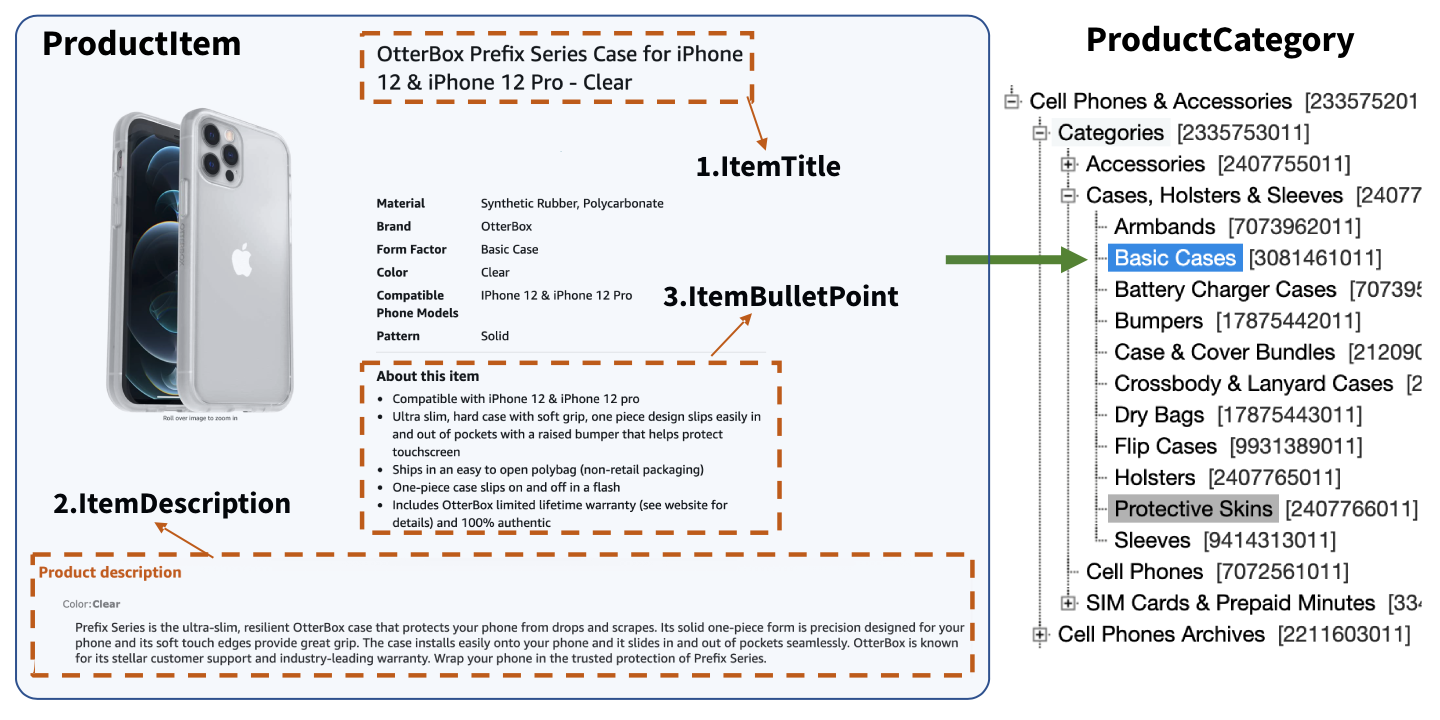
\includegraphics[width=0.8\linewidth]{figures/Data_Category-pdf.png}
    \caption{product item and category taxonomy}
    \label{fig:itemexample}
\end{figure}

\section{Product Data Quality and Noises}\label{sec:noise}
In this section, we will briefly introduce the common types of data noises that affect our classification model. The models of this study are based on natural language processing. Here, we only focus on the noise in text information, e.g. descriptions of items and semantic definitions of their categories. These types of noise are also prevalent in multi-modal data but differ in their manifestation and noise distribution. 

The text data of a product generally contains descriptions of the item properties. The product title information includes the major properties and functions of the item as a single sentence. Sometimes, the item’s category name is already provided in the title. A more detailed description of the product, its various functions and properties is usually found in the item description in the form of several sentences or bullet points. Thus, sentence-level semantic understanding is crucial to extract the full value of this information. It is worth noting that all of the aforementioned data noise comes from the large raw data mostly provided by sellers, hence manual cleaning requires significant cost and time. 

Item categories are predefined by online retailers according to catalog selection. The structure of categories, also termed as taxonomy, is the label space that we are targeting during classification. Hence, given different taxonomies, the accuracy of classification models varies due to changes in the complexity and dimension of the label space. In general, a taxonomy is manually curated by taxonomists as a hierarchical tree. Its granularity decides the size of item categories and learning logic from a given root node to its leaf children. Due to the selection are localized, taxonomy trees are not consistent across locales, thus a model capable of handling various label spaces is needed. 

\subsection{Incomplete and Misleading Item Descriptions}
Incompleteness and misleading product description make the classification task challenging. In this study, we focus on three item text features: item title, item description and item bullet points. The information necessary for a correct classification might exist in each of them or across features. For example, in pet supplies, an aquarium mat, that should be classified as an aquarium decoration, might be confused with a dog bed mat, if the keyword ”aquarium” is missing in the title. It is a common case, especially in a new locale where low quality data samples are abundant. Sometimes, incomplete item description comes with misleading information, which results in additional confusion for the model. In the previous case, the item bullet points of the aquarium mat focus on how to clean this item, misleading the classifier on the product usage instead of what the product is, and classify it as an aquarium cleaner. This problem might be severe if the other features are short or noisy. Another example is a fish tank which contains several aquarium decorations as gifts. The model needs adaptive ability to focus on important descriptions of the main product in a bundle. 


\subsection{Adversarial Item Information}
This type of data noise is generated by the sellers who might change item descriptions to depict different product aspects, intentionally or not, leading to products potentially depicted for a different category. We can further characterize the noise into soft adversarial noise and hard adversarial noise. The soft adversarial noise emphasizes some peripheral properties of the item, while the hard adversarial noise contains mendacious item descriptions. In the former scenario, to increase the visibility of their products, some sellers tend to describe multiple functions or properties of the item in detail, which obscures its inherent purpose. It is analogous to the case of misleading item description discussed before. This noise increases the difficulties of a stable learning. In the latter scenario, item description is totally irrelevant to the actual selling item. For instance, a TV mount frame can camouflage as a TV with various sizes as long as the seller removes the keyword ”mount” from the title. Interestingly, this type of adversarial noise sometimes couples with a correct item image, which suggests opportunities to introduce multimodal learning (such as using product images)  during product classification.           

\subsection{Definition of Noise in Label Space}
Another important yet hard to eliminate data noise is label noise. Unlike in the unsupervised setting, where the label space can be inferred during feature learning, we train our classifier with supervised knowledge. This label space is constructed by taxonomists from a selected group of samples over a period of time, or inherited or migrated from an established stable ontology, e.g. item categories of a new locale is a child tree of a mature locale on an international online retailer. As data accumulates, the amount of items with previously unseen labels increases and thus the current taxonomy fails to capture the true label complexity. On the other hand, defined labels are not necessarily mutually exclusive, resulting in a multi-label learning problem. However, incomplete label space is inevitable in this setting. Confusing labels present additional difficulties for supervised classification. 




\section{Deep Hierarchical Product Classification Framework (DHPC)}
The proposed model for product classification is a two-stage classifier, making the whole pipeline work as a hierarchical classifier. There are two main reasons. First, the label space of target product categories contains thousands of labels, which are sometimes confusing. Some techniques termed as extreme multilabel classification/ranking (XML/XMR) are designed to deal with this type of learning tasks with large label space. However, effective information mining from the large noisy dataset poses numerous challenges to reach high accuracy. The other reason for hierarchical classification is that taxonomy structure defined by internal taxonomists is a hierarchical tree. It is straightforward to incorporate this structure into our model. Besides, from the business perspective, a hierarchical classifier can help to identify departments with low accuracy and then to fine-tune them separately in the order of priority. In this paper, we denote the first level classifier as the department classifier, which assigns products to a department, e.g., electronics, fashion etc. Each locale generally contains dozens of departments. The second level classifier, called a leaf classifier, predicts items further into granular categories of each department. The number of categories ranges from hundreds to tens of thousands. 

The whole pipeline is shown in Fig.~\ref{fig:pipeline}. First, item text information including item title, description and bullet points are preprocessed to remove nonalphabetic characters and resample for balanced category distribution. Since the number of categories in department and leaf classifiers are distinct, we shall wisely select sampling threshold values. For department classifier, we randomly select hundreds of items per leaf node and combine all leaf node samples in a given department. For leaf classifier, we randomly select thousands of items per leaf node without replacement. After data preprocessing, the department and leaf classifiers are trained independently with an identical deep network structure. Details of the model structure will be presented in the next section. 

The inference pipeline differs from the training schedule. Rather than independent querying, it works in cascade from department prediction down to leaf node prediction. As indicated in Fig.~\ref{fig:pipeline}, the department classifier predicts the source item into the electronics department. The leaf classifier of the electronics department further predicts that item as a iPhone case. That is, we rank model prediction scores to find suggested department and then infer a leaf node within that department. During this process, a set of department prediction scores and the corresponding set of leaf prediction scores is generated. The two scores are then multiplied as confidence score for thresholding and model calibration. 

\begin{figure}[h]
\center
        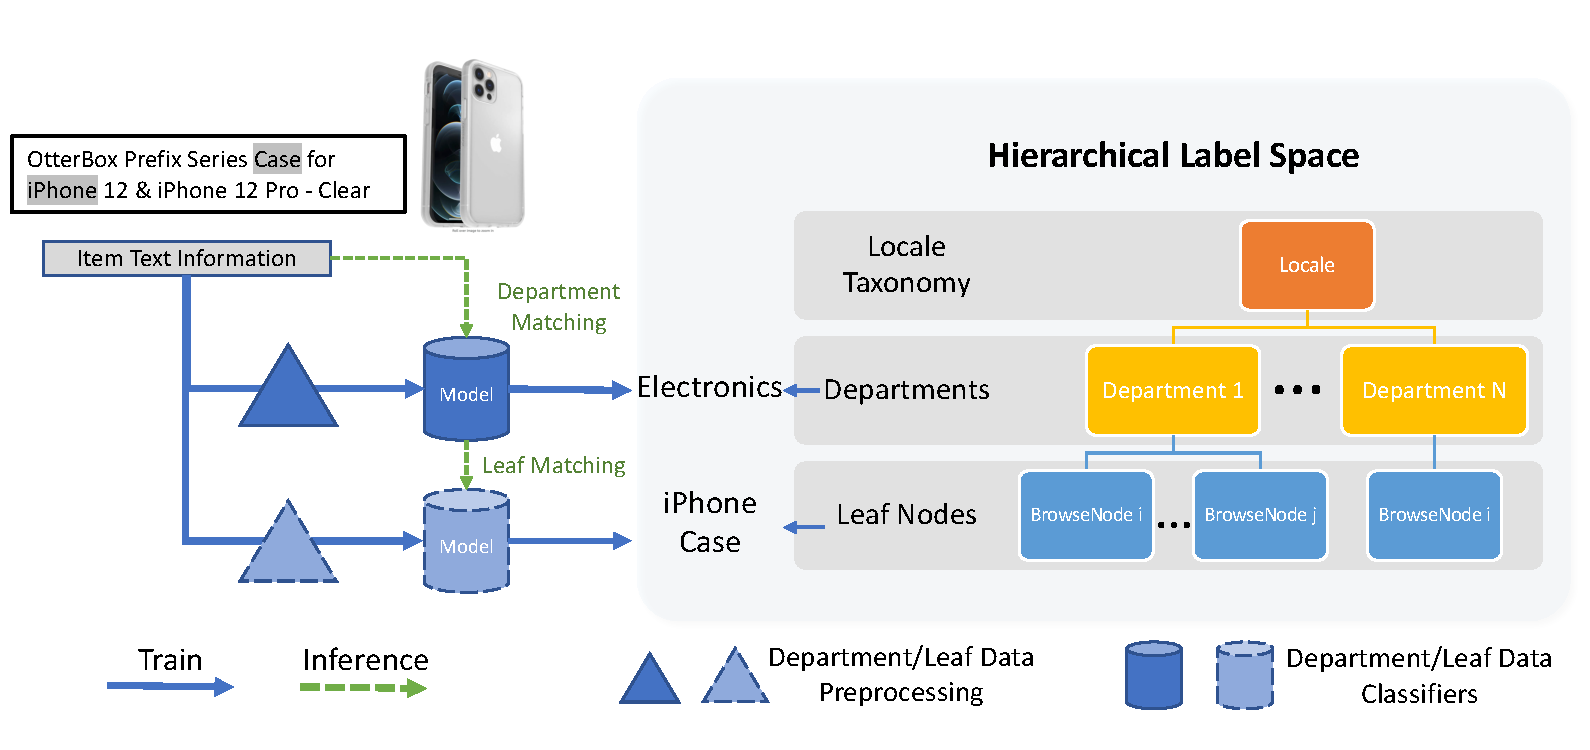
\includegraphics[width=0.9\linewidth]{figures/Pipeline_general.pdf}
    \caption{Hierarchical product classification framework (DHPC). The blue arrow and green arrow streams respectively indicate training and inference processes.}
    \label{fig:pipeline}
\end{figure}

\begin{figure}[h]
\center
        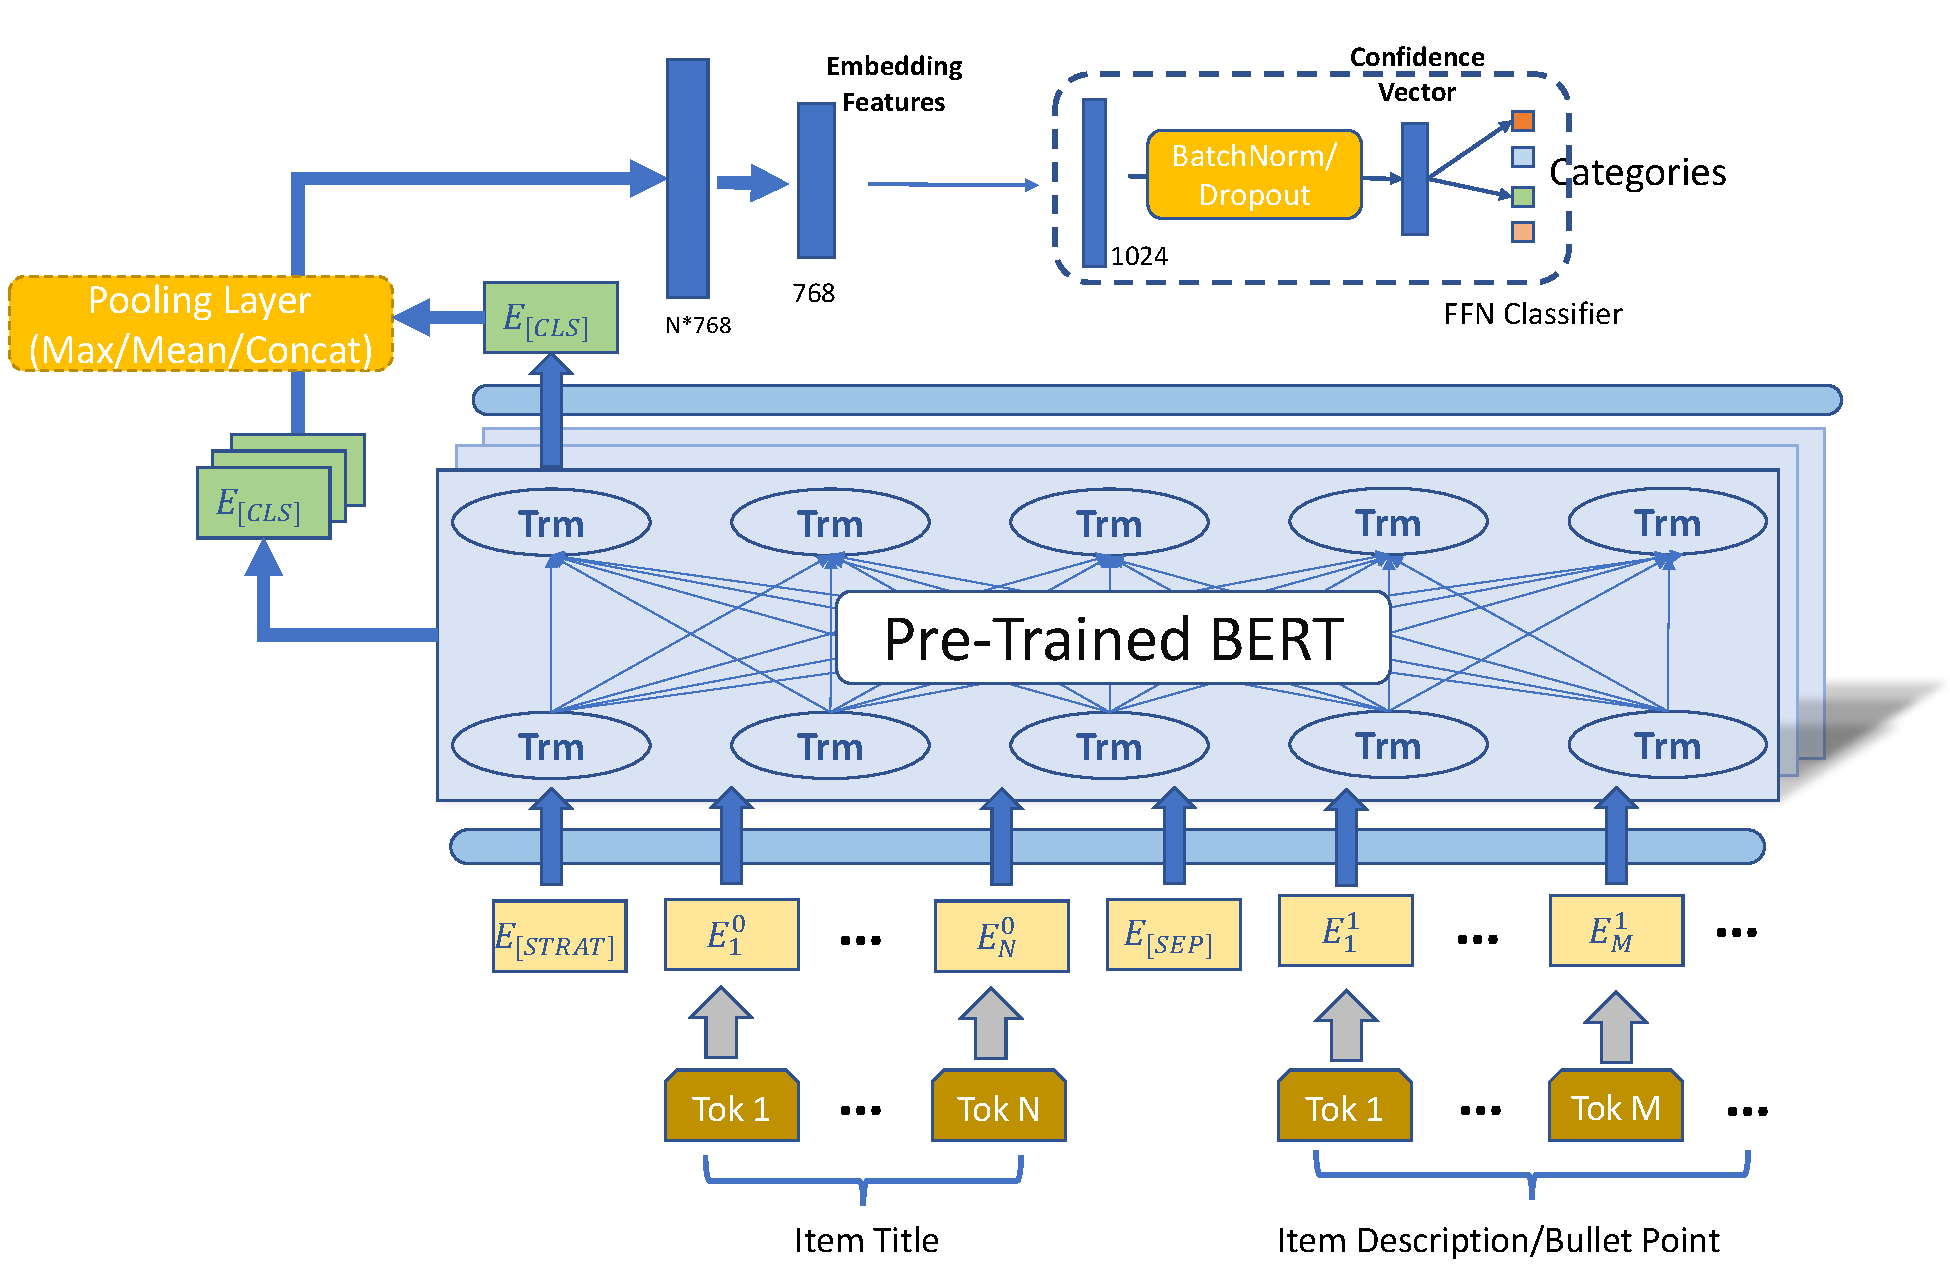
\includegraphics[width=0.8\linewidth]{figures/Model_structure.pdf}
    \caption{Deep hierarchical product classifier with pre-trained BERT knowledge}
    \label{fig:bertmodel}
\end{figure}





\subsection{Deep Neural Network Classifier}
Considering model ability to handle multiple languages for various locales, we select a state-of-the-art multilingual model as the backbone structure. Specifically, we choose to use the pre-trained Bidirectional Encoder Representations from Transformers (BERT) in a multilingual setting. Our model is then fine-tuned on top of this architecture with an additional feed-forward neural network (FFNN) as the non-linear classifier. The model architecture is shown in Fig.~\ref{fig:bertmodel} and consists of 4 important components: an embedding component, an transformer encoder, a feature pooled network and a non-linear multi-layer classifier. Parameters of the embedding component and transformer encoder are pre-trained on a large corpus of multilingual text.

In the first step, item text information is tokenized by a trained multilingual dictionary (contains 30522 words). Then, the embedding layer projects these tokenized words into a latent space. WordPiece embedding is used here instead of the usual practice word embedding. During this process, segment embedding and position embedding are also concurrently encoded and added to the token embedding. It allows the model to understand sentence-wise sequential order. In our case, we use segment embedding to indicate whether words belong to item title, description or bullet points. The output of this embedding layer is a sequence of high dimensional symbol representations.

The transformer encoder maps the output of the embedding layer to a sentence/paragraph level semantic embedding vector, $E_{[CLS]}$. The original BERT transformer encoder contains 12 identical bidirectional transformer layers. Each layer has two sub-layers. The first is a multi-head self-attention mechanism, and the second is a simple, position-wise fully connected FFNN. A residual connection is employed around each of the two sub-layers, followed by layer normalization. That is, the output of each sub-layer is LayerNorm(x+Sublayer(x)). 

\stitle{Knowledge Skip.} Generally, supervised classification tasks use the first embedding vector $E_{[CLS]}$ of outputs of the transformer layer as the semantic representation. During experiments, we observed that keywords of product categories frequently exist in the title information, which is relatively easier to catch by attention than statement understanding. Therefore, in our model, we consider both deep and shallow encoded knowledge to enhance classification accuracy. $E_{[CLS]}$ from every other intermediate transformer layer are pooled together with the last one and then undergo a feature pooling network. There are several options for feature pooling, e.g., maxpool, meanpool or concatenation. 

% We evaluate each of the strategies in the experiments. Due to the complexity of different department classifiers, we choose to concatenate all $E_{[CLS]}$ and eventually obtain an embedding feature vector of the same dimension as $E_{[CLS]}$.

The last part of our model is a two-layer fully-connected network with BatchNorm and Dropout layers inside. The classification loss is binary cross entropy allowing for multi-label learning.

\subsection{Model Accuracy and Coverage}
Model accuracy and coverage are two essential evaluation metrics we use to quantitatively assess the model performance in a product classification system. Since the ground truth distribution of product categories is unequal, and the importance of categories is determined by business purposes, the preferred model must combine high accuracy with high coverage. 

\section{Training Strategy}\label{sec:training}
Training a deep neural network on large noisy data, e.g. classifying millions of items with thousands of target labels, would easily result in overfitting and get trapped in a false local optimum, i.e. overconfidence. Especially in our cases, the product's text information contains mixed types of noise mentioned in the Sec.~\ref{sec:noise}. To overcome these difficulties during the training process, general training strategies, such as early stopping, dropout, weight regularization/decay etc., are employed. Moreover, to further improve the model as well, we adopt the following training strategies.   


\subsection{Bootstrap Learning}
The first training strategy is a self-justified learning mechanism accounting for knowledge consistency during training~\cite{reed2014training}. It augments the usual prediction objective with a notion of perceptual consistency, e.g. consistency of model predictions in each batch training. More specifically, it allows the model to disagree with a perceptually-inconsistent training label and effectively relabel the data while training. The assumption behind this idea is that incorrect labels are likely to be inconsistent with other data points predicted to the same label by the model. Therefore, it acts in a manner of self label clean-up and bootstraps itself until convergence to a stable knowledge. Here, we incorporate this idea into the cross-entropy training loss. Recalling the binary cross-entropy (BCE) loss:

\begin{equation}\label{eq:bce}
    L_{BCE}(p,q) = -\sum_{k=1}^{N}p_klog(q_k)+(1-p_k)log(1-q_k),
\end{equation}
where $p_k, q_k$ are ground truth label and model prediction, respectively. $N$ is the size of target labels. To allow for differentiability of the proposed bootstrap loss, the label consistency is defined by predicted category probabilities $q_k$, hence the above BCE loss is modified as:

\begin{equation}\label{eq:bootstrap}
    L_{Bootstrap}(p,q) = -\sum_{k=1}^{N}\beta p_klog(q_k)+\beta (1-p_k)log(1-q_k)+ (1-\beta)q_klog(q_k),
\end{equation}
where parameter $0\leq\beta\leq1$ balances bootstrap learning and supervised classification. It is empirically set in the range $[0.8, 0.95]$. Due to the large batch training steps ($t_{batch}$), we can set a delta activation $\hat{\beta}$ that adaptively turns on/off the bootstrap loss at a given global step $T_{gate}$:
\begin{equation}
    \hat{\beta}= \left \{
  \begin{aligned}
    &1, && \text{if}\ t_{batch}<T_{gate}\\
    &\beta, &&\text{if}\ t_{batch}\geq T_{gate}\\
  \end{aligned} \right.
\end{equation}

\subsection{Negative Sampling}\label{sec:negsamp}
It is common that a product possess multiple functions, but we have limited knowledge of their complete category labels in the training data. The label tags are provided by sellers based on their limited knowledge of category taxonomy. Generally, one or a few positive labels will be allocated for a given item in the training set and the rest of labels are assumed to be negatively associated with it. However, in such a setting, negative samples outnumber positive samples dramatically, leading to a high precision but low recall. To avoid quick convergence to a false local optimum, we adopt negative sampling in the learning objective. Suppose, in Eq.~\ref{eq:negsamp}, $N=N_{pos}+N_{neg}$, i.e., $N_{pos}$ positive labels and $N_{neg}$ negative labels. Eq.~\ref{eq:bootstrap} is updated as:
\begin{equation}\label{eq:negsamp}
    L_{negsamp}(p,q) = -\sum_{k=1}^{N_{pos}}\hat{\beta} p_klog(q_k)-\frac{N_{neg}}{\sigma N}\sum_{j\sim P(\sigma)}^{N_{neg}}\hat{\beta} (1-p_k)log(1-q_k)- \sum_{k=1}^{N}(1-\hat{\beta})q_klog(q_k),
\end{equation}
where $P(\sigma)$ is a probability function to select soft negative samples, and $\sigma$ controls their contribution in the loss.    


\subsection{Soft Label with Temperature Scaling}
Label smoothing is a way to make our model more robust so that it generalizes well, which is especially useful in big data mining. It was first introduced by Szegedy et al.~\cite{szegedy2016rethinking} for multi-class supervised learning tasks in computer vision. It is originally designed for the last classifier layer with softmax function to prevent overconfidence. The mathematical formulation is simple:
\begin{equation}
    p_k=(1-\epsilon)p_k+\epsilon u(k),
\end{equation}
by mixing the ground truth label $p_k$ with a scaling term $u(k)$. $u(k)$ is a distribution function in the label space and the simplest choice is a fixed scaling value, e.g. $\frac{1}{N}$. Hence, it prevents the largest logit (output of last layer) from becoming much larger than all others. We use a similar idea to scale prediction scores instead of the ground truth labels. In Eq.~\ref{eq:negsamp}, $q_k$ is the sigmoid output of logit, $q_k=sigmoid(logit_k)$. Therefore, following the same logic, we modify $q_k$ as :
\begin{equation}
    q_k=sigmoid(\frac{logit_k}{\epsilon(t_{batch})}),
\end{equation}
where $\epsilon>0$ can be a fixed value or a function of global batch training step $t_{batch}$ allowing for adaptive scaling as we did in $\hat{\beta}$. It is worth noting that $\epsilon>1$ and $\epsilon<1$ carries quite different roles during training, forcing the model towards the opposite converging status. Setting $\epsilon>1$ in the early training stage can help to explore potential local optima while setting $\epsilon<1$ makes the model quickly converge to a local optimum.


\subsection{Augmentation with Label Semantic Information}
Label semantic information plays an essential role in product classification, since this knowledge is predefined to perceptively group items with their inherent properties. We also observe that, if text information of an item contains key words having a similar morphology of label name, it has a greater chance to be correctly predicted. Hence, we believe it is beneficial to incorporate the label information into our training data and force the model to understand these patterns. 
Specifically, we randomly chose a small portion of training data per leaf node and shuffling their title information by words. Then, we insert their labels' name in any place of the shuffled title. Their item description and bullet points are removed. Because, comparing with item title, other text information tend to follow the logic of natural language in sentences. Shuffling would destroy these properties.

 

\section{Experiments}
In this section, we include several experiments to validate the effectiveness of the proposed framework in two large datasets. We also conduct an analysis of product classification with different data settings, model structures, supervised learning goals and training strategies. Since these factors might positively affect our supervised learning tasks, we explore their potential and use cases. All experimental details are given below and results are reported with discussions.

\subsection{Product Classification in 2 Large Datasets}
This experiment is designed to evaluate the proposed model in real use cases. We try to understand how it performs under different language environments and data qualities.  

\subsubsection{Experimental Settings}
 Two independent datasets are sampled from two European locales (two countries, L1 and L2, using distinct languages from an online retailer) which contain millions of product items with text information in a newly build online shopping site. L1 data contains $50\%$ of golden data source, i.e. positive labels of items were human-audited and hence high quality, and $50\%$ general data, i.e., samples of original product data source with noise. L2 data is all general data which means it is noisier than L1 data. The major challenge of learning with these two datasets is that we do not have complete positive/negative label information for each item, e.g. labels are not fully explored. Discussion of data collections and label process can be found in Sec.~\ref{sec:noise} and Sec.~\ref{sec:negsamp}. The training data contains several hundreds of millions of items with thousands of labels. The test set for each locale is sampled from catalog based on importance. It contains thousands of items distributed in thousands of labels. For these datasets, the text information is mixed with incomplete data source (i.e. missing item description or bullet point) that are deliberately constructed to assess practical use cases. 
 
%  General data information is reported in Tab.~\ref{tab:datasource}.  Therefore, it contains less but import leaf node samples than the training data. Besides, we indicate data heterogeneity in Tab.~\ref{tab:datasource}, in terms of the percentage of how many training items have 3-views of text information (title, description, and bullet point).     

We chose a deep neural network (DNN) model as the baseline comparison. It encodes multi-view text inputs through an embedding layer and then pools the embeddings before a Multilayer Perceptron Classifier (MPC). The MPC consists of a few fully connected layers. This simple yet effective model successfully classify product item with high accuracy. It worth noting that the DNN model is trained from scratch for each dataset using the same set of hyper-parameters.   

Accuracy score is calculated from the human assessment of the model prediction. The final prediction score is the multiplication of department confidence score and leaf confidence score, reflecting how much confidence a model has in the final leaf node predictions. This score is then used to threshold model prediction in order to reach a given accuracy demand. Please note, all of the assessment is weighted by the importance of departments.



\begin{table}[]
    \centering
    \caption{Comparison with DNN baseline model for department/leaf classification in the L1 data. Improvement(+)/Downgrade(-) of the department/leaf level accuracy is reported.}
    \resizebox{0.7\textwidth}{!}{
\begin{tabular}{lrrr}
\toprule
                           Department Name &  Department Acc Improve &  Leaf Acc Improve  \\
\midrule
                         Department 1 &            -0.0377 &           -0.0427              \\
                        Department 2 &            -0.1230 &            +0.0258              \\
     Department 3 &            -0.0254 &            +0.0317             \\
         Department 4 &            +0.0065 &           -0.0433          \\
                 Department 5 &            -0.0506 &            +0.0148            \\
 Department 6 &            -0.0578 &            +0.0599          \\
                Department 7 &            -0.0262 &            +0.0520            \\
                Department 8 &             +0.0016 &            +0.0819           \\
                      Department 9 &            -0.0249 &            +0.0253           \\
                  Department 10 &            -0.0658 &           -0.0067            \\
                          Department 11 &             +0.0182 &            +0.0173            \\
                       Department 12 &             +0.0321 &            +0.0771           \\
\bottomrule
\end{tabular}}
    \label{tab:NL_results}
\end{table}




\subsubsection{Results}
\stitle{L1 Dataset.} Hierarchical classification results of product items in L1 are shown in Tab.~\ref{tab:NL_results}. Compared with the DNN baseline, the overall accuracy predicted by the proposed model is improved by 3.4\% for leaf node predictions but slightly worse (drops 1\%) for department predictions. Considering the chain effect in the hierarchical classification, within some departments, DHPC possesses a significantly better accuracy than the DNN model. For example, in Department 11 (the largest department) and Department 12 (the 3rd largest), DHPC is better in both department and leaf classifiers. However, we also observe that, in the 2nd largest department (Department 4), although the department classification beats DNN model, DHPC has an obvious worse accuracy in leaf node classification. After investigation, we found the discrepancy is caused from resampling strategies during data prepossessing since category distribution in this department is less balanced than in the other 2 largest departments. 

\stitle{L2 Dataset.} L2 data is generally noisier than L1 data, hence the overall classification accuracies in the department and leaf level are lower than that of L1 product classification. In comparison, DHPC improves leaf node accuracy by 2\% while the department level accuracy remains the same. Similarly, we further compare them in Department 3, 4, 6 (the top-3 largest departments). Except for the department classification of Department 3, all of the other department/leaf classifications indicate superior performance of the proposed model. Overall, DHPC excels in most department and leaf classifications in the L2 dataset.

\stitle{Accuracy VS. Coverage.} In addition to the accuracy assessed with the whole dataset, we attempt to evaluate the confidence of the proposed model, providing insights for model fine-tuning. To this end, we threshold model predictions based on confidence scores to allow at least 90\% accuracy. For L1 dataset, DHPC outperforms DNN model by 13\% more coverage after thresholding. For L2 dataset, we observe 13\% more coverage at 90\% accuracy compare to the DNN model. 




\begin{table}[]
    \centering
    \caption{Comparison with DNN baseline model for department/leaf classification in L2 data.}
    \resizebox{0.65\textwidth}{!}{
\begin{tabular}{lrrr}
\toprule
                    Department Name &  Department Acc Improve &  Leaf Acc Improve  \\
\midrule
              Department 1 &            -0.1516 &            +0.0345          \\
              Department 2 &             +0.0324 &            +0.0231 \\
Department 3 &            -0.0338 &            +0.0252  \\
                          Department 4 &             +0.0091 &            +0.0259  \\
           Department 5 &             +0.0511 &            +0.1128  \\
                     Department 6 &             +0.0085 &            +0.0441  \\
            Department 7 &            -0.0477 &           -0.0630  \\
              Department 8 &             +0.0909 &            +0.0489  \\
     Department 9 &            -0.0607 &           -0.0643  \\
               Department 10 &             +0.0417 &            +0.0913  \\
\bottomrule
\end{tabular}}
    \label{tab:SE_results}
\end{table}




\subsection{Ablation Study of Proposed Training Strategies}
In this section, we conduct several ablation studies to evaluate our proposed training strategies and discover their potentials. Parameter exploration in these experiments provides hints for future model design.

\subsubsection{Evaluation of Active Bootstrap Learning}
Active bootstrap learning helps the model to capture the most consistent knowledge (self-confidence) during training and overcome overfitting issues. We explore various parameter choices for the L1 department classifier. $\beta$ controls the strength of self-confidence. $T_{gate}$ indicates at which global training step we will turn on this strategy, otherwise the model uses the traditional binary cross-entropy loss. From results in Tab.~\ref{tab:bootstrap}, we find early initialization of bootstrap learning, e.g. $T_{gate}=0$ with a weak self-confidence setting, e.g. $\beta=0.9$, offers the best performance. Hence, we argue that, for product classification, consistent knowledge captured at the very early stage of training contributes to high accuracy predictions.

\begin{table}[h]
    \centering
    \caption{Influence of bootstrap learning in L1 department classification. Improvement (+) or Downgrade (-). }
    \resizebox{0.5\textwidth}{!}{
\begin{tabular}{c|cccc}
% {lrrrr}
\toprule
            $\beta$ &   0.9 &  0.8 &  0.7 &  0.6  \\
\midrule
              $T_{gate}$ = 0 &         \textbf{+0.0148} &        -0.0016 &     +0.0047 &    +0.0029      \\
              $T_{gate}$ = 1000 &         \textbf{+0.0007} &        -0.0015 &     -0.0023 &    -0.0038        \\
            $T_{gate}$ = 3000 &         \textbf{-0.0011} &        -0.0020 &     -0.0024 &    -0.0038        \\
\bottomrule
\end{tabular}}
    \label{tab:bootstrap}
\end{table}



\subsubsection{Model Pruning}
We prune the original BERT model structures by using shallow embedding features for product classification. Specifically, we extract $E_{[CLS]}$ of the first 2 layers and then pooling ($PruneBert_2$), first 4 layers ($PruneBert_4$) and first 6 layers ($PruneBert_6$). We follow the same hyper-parameter settings for all pruned models and test their prediction power in two L1 product classification tasks, e.g., department classification and leaf node classification of Department 10. In this experiment, we do not add any noise handling training strategies introduced in Sec.~\ref{sec:training}. The prediction accuracy is reported in Tab.~\ref{tab:modelprune}, which indicates a very close performance to the original BERT when using its first 4 layers. Considering that the original BERT has 110 MM parameters, this experiment suggests a simple structure of BERT with shallow encoding layers (half of total parameters) while effectively captures categorical information in our tasks.    


\begin{table}[]
    \centering
    \caption{Changes of department/leaf prediction accuracy after model pruning.}
    \resizebox{0.6\textwidth}{!}{
\begin{tabular}{c|ccc}
% {lrrrr}
\toprule
            Model &  $PruneBERT_2$ &  $PruneBERT_4$ &  $PruneBERT_6$   \\
\midrule
              Department Classifier (L1) &         -0.012 &        -0.004 &     -0.003         \\
              Leaf Classifier (Department 10, L1) &         -0.015 &        -0.001 &     -0.003     \\
\bottomrule
            Parameters & 40MM   & 54MM  & 67MM \\
\bottomrule
\end{tabular}}
    \label{tab:modelprune}
\end{table}


\subsubsection{Evaluation of Negative Sampling}
Defining a suitable $P(\sigma)$ in Eq.~\ref{eq:negsamp} is challenging given the complex confusion patters across departments. In this preliminary study, we randomly select a portion of unlabeled categories ($\sigma$) as soft negative labels. Here, we explore $\sigma$ settings from 0 to 60\% with step size 10\% for department and leaf classifiers respectively. As shown in Tab.~\ref{tab:negsamp}, the department classifier exerts the best performance when negative sampling is turned off, but the leaf node classifier embraces a large $\sigma$ value, e.g. $\sigma=0.7$ for leaf classifier of Department 10 in L1 data. 

\begin{table}[]
    \centering
    \caption{Influence of negative sampling in department/leaf classification. Improvement (+) or Downgrade (-). }
    \resizebox{0.5\textwidth}{!}{
\begin{tabular}{c|ccccc}
% {lrrrr}
\toprule
            $\sigma$ &  0.9 &  0.8 &  0.7 &  0.6  \\
\midrule
              Department Classifier (L1) &          -0.013 &        -0.019 &     -0.011 &    -0.019      \\
              Leaf Classifier (Department 10, L1) &         +0.006 &    +0.001 &     \textbf{+0.010} &    +0.005     \\
\bottomrule
\end{tabular}}
    \label{tab:negsamp}
\end{table}


\subsubsection{Evaluation of Soft Labels}
We search smoothing factor $\epsilon$ in a wide range [1.5, 0.7] to provide a comprehensive understanding of soft labels for noisy data. We turn on this strategy at the very beginning of the training process since we do not found any opportunities if we delay it. The result in Tab.~\ref{tab:labelsmooth} shows that making smoothed soft labels, e.g., $\epsilon<1$, helps our model towards high accuracy but it has to be carefully chosen to prevent from over-smoothing, e.g. downgrade if $\epsilon<0.7$. We also find the necessity of more training epochs to allow a complete convergence (20\% more training epochs).


\begin{table}[h]
    \centering
    \caption{Influence of soft label in department/leaf classification. Improvement (+) or Downgrade (-). }
    \resizebox{0.5\textwidth}{!}{
\begin{tabular}{c|cccc}
% {lrrrr}
\toprule
            $\epsilon$ &  1.5 &  1.2 &  0.9 &  0.7  \\
\midrule
              Department Classifier (L1) &         -0.002 &        -0.001 &     \textbf{+0.015} &    +0.005      \\
              Leaf Classifier (Department 10, L1) &         -0.010 &        +0.001 &     \textbf{+0.010} &    -0.002      \\
\bottomrule
\end{tabular}}
    \label{tab:labelsmooth}
\end{table}


\section{Conclusions and Future Work}
In this study, we propose a deep hierarchical classification framework for text-based product classification based on the pre-trained multilingual BERT model. We address typical types of data noises in the product data source and design several learning strategies to handle them. Experiments on two large datasets demonstrate the effectiveness of the proposed model. The additional ablation study further provides domain knowledge of optimal choices of training strategies under different data and task settings. 

There are several interesting directions for further investigation. For example, we can improve classification accuracy by using a pre-trained model designed for languages of the targeting locale. Besides, multimodal information such as product images can be complementary sources as a feature. In addition, we can further upgrade the proposed training strategies by adding/replacing them with self-adaptive selection functions, such as label-semantic-based negative sampling.    








% \section*{Acknowledgments}

  
% \newpage

%\bibliographystyle{IEEEtran}
%\bibliography{abbreviations}

% Generated by IEEEtran.bst, version: 1.14 (2015/08/26)
\providecommand{\noopsort}[1]{}
\begin{thebibliography}{10}
\providecommand{\url}[1]{#1}
\csname url@samestyle\endcsname
\providecommand{\newblock}{\relax}
\providecommand{\bibinfo}[2]{#2}
\providecommand{\BIBentrySTDinterwordspacing}{\spaceskip=0pt\relax}
\providecommand{\BIBentryALTinterwordstretchfactor}{4}
\providecommand{\BIBentryALTinterwordspacing}{\spaceskip=\fontdimen2\font plus
\BIBentryALTinterwordstretchfactor\fontdimen3\font minus
  \fontdimen4\font\relax}
\providecommand{\BIBforeignlanguage}[2]{{%
\expandafter\ifx\csname l@#1\endcsname\relax
\typeout{** WARNING: IEEEtran.bst: No hyphenation pattern has been}%
\typeout{** loaded for the language `#1'. Using the pattern for}%
\typeout{** the default language instead.}%
\else
\language=\csname l@#1\endcsname
\fi
#2}}
\providecommand{\BIBdecl}{\relax}
\BIBdecl

\bibitem{reed2014training}
Reed, Scott, Honglak Lee, Dragomir Anguelov, Christian Szegedy, Dumitru Erhan, and Andrew Rabinovich. "Training deep neural networks on noisy labels with bootstrapping." arXiv preprint arXiv:1412.6596 (2014).

\bibitem{szegedy2016rethinking}
Szegedy, Christian, Vincent Vanhoucke, Sergey Ioffe, Jon Shlens, and Zbigniew Wojna. "Rethinking the inception architecture for computer vision." In Proceedings of the IEEE conference on computer vision and pattern recognition, pp. 2818-2826. 2016.

\bibitem{pennington2014glove}
Pennington, Jeffrey, Richard Socher, and Christopher D. Manning. "Glove: Global vectors for word representation." In Proceedings of the 2014 conference on empirical methods in natural language processing (EMNLP), pp. 1532-1543. 2014.

  
\bibitem{bojanowski2017enriching}
Bojanowski, Piotr, Edouard Grave, Armand Joulin, and Tomas Mikolov. "Enriching word vectors with subword information." Transactions of the Association for Computational Linguistics 5 (2017): 135-146.

\bibitem{peters2018deep}
Peters, Matthew E., Mark Neumann, Mohit Iyyer, Matt Gardner, Christopher Clark, Kenton Lee, and Luke Zettlemoyer. "Deep contextualized word representations." arXiv preprint arXiv:1802.05365 (2018).

\bibitem{radford2018improving}
Radford, Alec, Karthik Narasimhan, Tim Salimans, and Ilya Sutskever. "Improving language understanding by generative pre-training." (2018).


\bibitem{radford2019language}
Radford, Alec, Jeffrey Wu, Rewon Child, David Luan, Dario Amodei, and Ilya Sutskever. "Language models are unsupervised multitask learners." OpenAI blog 1, no. 8 (2019): 9.

\bibitem{brown2020language}
Brown, Tom B., Benjamin Mann, Nick Ryder, Melanie Subbiah, Jared Kaplan, Prafulla Dhariwal, Arvind Neelakantan et al. "Language models are few-shot learners." arXiv preprint arXiv:2005.14165 (2020).

\bibitem{devlin2018bert}
Devlin, Jacob, Ming-Wei Chang, Kenton Lee, and Kristina Toutanova. "Bert: Pre-training of deep bidirectional transformers for language understanding." arXiv preprint arXiv:1810.04805 (2018).

\bibitem{taylor1953cloze}
Taylor, Wilson L. "“Cloze procedure”: A new tool for measuring readability." Journalism quarterly 30, no. 4 (1953): 415-433.

\bibitem{hinton2015distilling}
Hinton, Geoffrey, Oriol Vinyals, and Jeff Dean. "Distilling the knowledge in a neural network." arXiv preprint arXiv:1503.02531 (2015).

\bibitem{liu2017deep}
Liu, Jingzhou, Wei-Cheng Chang, Yuexin Wu, and Yiming Yang. "Deep learning for extreme multi-label text classification." In Proceedings of the 40th International ACM SIGIR Conference on Research and Development in Information Retrieval, pp. 115-124. 2017.

\bibitem{jain2016extreme}
Jain, Himanshu, Yashoteja Prabhu, and Manik Varma. "Extreme multi-label loss functions for recommendation, tagging, ranking \& other missing label applications." In Proceedings of the 22nd ACM SIGKDD International Conference on Knowledge Discovery and Data Mining, pp. 935-944. 2016.

\bibitem{goldberg2014word2vec}
Goldberg, Yoav, and Omer Levy. "word2vec Explained: deriving Mikolov et al.'s negative-sampling word-embedding method." arXiv preprint arXiv:1402.3722 (2014).

\end{thebibliography}

\end{document}